\section{The Hash-and-Resubmit Pattern}

We now introduce a novel design pattern for Solidity smart contracts which
results into massive gas optimization due to the elimination of expensive
storage operations.

\textbf{Motivation.}
% This part is maybe too shallow. Consider deleting it. >>>> In the Ethereum
% blockchain, Turing-complete smart contracts were introduced. In order to
% prevent accidental or adversarial DoS phenomena such as infinite loops of
% code, contract invocations are bounded by an amount of gas units~\cite{wood,
% buterin}.  <<<<
It is essential for smart contracts to store data in the blockchain. However,
interacting with the storage of a contract is among the most expensive
operations of the EVM~\cite{wood, buterin}. Therefore, only necessary data
should be stored and redundancy should be avoided when possible. This is
contrary to conventional software architecture, where storage is considered
cheap. Usually, the performance of data access in traditional systems is
related with time.  However, in Ethereum performance is related to gas
consumption. Access to persistent data costs a substantial amount of gas, which
has a direct monetary value. One way to mitigate gas cost of reading variables
from the blockchain is to declare them public.  This leads to the creation of a
\emph{getter} function in the background, allowing free access to the value of
the variable. But this treatment does not prevent the initial population of
storage data, which is significantly expensive for large size of data.
Towards the goal of implementing gas-efficient smart contracts, several
patterns have been proposed~\cite{contract-opt-1, contract-opt-2,
contract-opt-3}.

By using the \emph{hash-and-resubmit} pattern, large storage variables are
omitted entirety, and structures are contained in memory which results to
vastly improved performance. When a function call is performed, the arguments
and signature of the function is included in the transactions field of the body
of a block. The contents of blocks are public to the network, therefore this
information is available to nodes. By simply observing blocks, a node retrieves
data sent by other users, which is processed off-chain. To interact with data
originated by other users, the node resends the observed information to the
public network, possibly accompanied by complementary data depending on the
context of the application. The concept of resending data would be redundant in
conventional systems. However, in Solidity this can be utilized very
efficiently because function arguments are contained in memory rather than
storage, which supports vastly cheaper operations.

\begin{figure*}[h]
    \begin{center}
        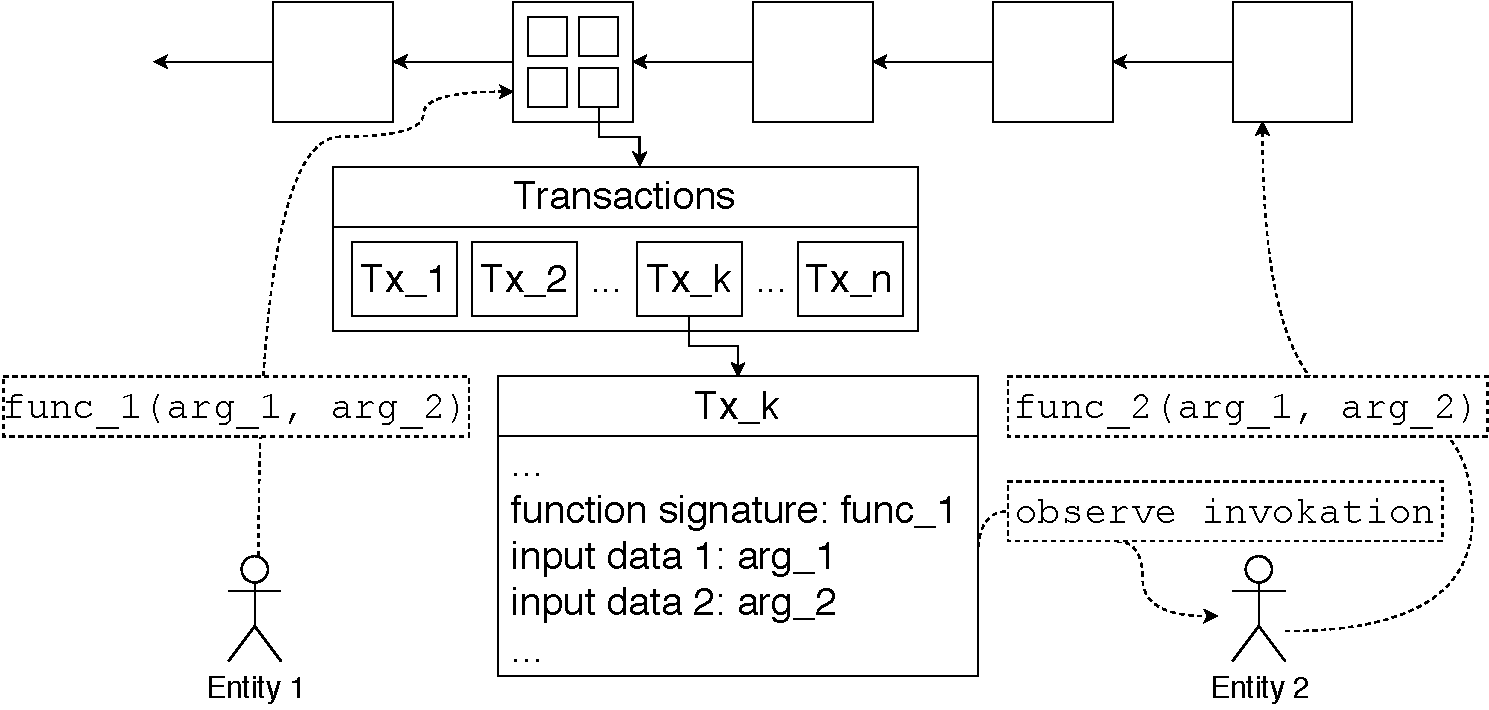
\includegraphics[width=1\textwidth]{figures/observer-tx.pdf}
    \end{center}
    \caption{Entity 1 makes a function call with arguments arg1 and arg2.
    Entity 2 reads the content of transactions in the block and retrieves the
    input data. Entity 2 can use this data to make a different invocation.}
    \label{fig:observe-tx}
\end{figure*}

\noindent
\textbf{Applicability.}
We now list the cases in which the \emph{hash-and-resubmit} pattern is
efficient to use:
\begin{enumerate}
    \item To reduce gas cost due to extensive read/write storage operations
        and to make smart contracts that exceed block gas limit practical.
    \item To interact with smart contract depending on prior actions of other
        users
    \item When a full node observes the traffic of a contract
\end{enumerate}

\newcommand{\proc}{\textsf{func}}

\noindent \textbf{Participants and collaborators.} The first participant is the
smart contract $\contract$ which accepts function calls. Another participant is
the invoker $\invoker$, who dispatches arbitrary data $\data_0$ to $\contract$
via a function \texttt{\proc$_1$}($\data_0$). Note that $\data_0$ are
potentially processed on-chain, resulting to $\data$. The last participant is
the observer $\observer$, who is a node that observes transactions towards
$\contract$ in the blockchain. After observation, $\observer$ retrieves data
$\data$. Finally, $\observer$ acts as an invoker by making a new interaction
with $\contract$, \texttt{\proc$_2$}($\data$). However, a malicious $\observer$
may alter $\data$ before interacting with $\contract$. We will denote the
potentially modified $\data$ as $\datas$. The verification that $\data =
\datas$, which is a prerequisite for the secure functionality of the underlying
contract consists a part of the pattern and is performed in
\texttt{\proc$_2$}($\datas$).

\noindent \textbf{Implementation.} The implementation of this pattern is
divided in two parts. The first part covers how $\datas$ is retrieved by
$\observer$, whereas the second part explains how the verification of
$\data=\datas$ is realized. The challenge here is twofold:

\begin{enumerate}

    \item Availability: $\observer$ must be able to retrieve $\data$ without
        the need of accessing on-chain data.

    \item Consistency: $\observer$ must be prevented from dispatching $\datas$
        that differs from the originally submitted $\data$.

\end{enumerate}

\noindent
\emph{Hash-and-resubmit} technique is performed in two
stages to face these challenges: (a) the \emph{hash} phase, which addresses
\emph{reliability}, and (b) the \emph{resubmit} phase which addresses
\emph{availability} and \emph{reliability}.

\noindent \textsf{Addressing availability:} During \emph{hash} phase,
$\invoker$ makes the function call \texttt{\proc}$_1$($\data_0$). This
transaction, which includes a function signature (\texttt{\proc$_1$}) and the
corresponding data ($\data_0$), is added in a block by a miner. Due to
blockchain's transparency, the observer of \texttt{\proc}$_1$, $\observer$,
retrieves a copy of $\data_0$, without the need of accessing contract data. In
turn, $\observer$ performs \emph{locally} the same set of on-chain instructions
operated on $\data_0$ generating $\data$.

\noindent \textsf{Addressing reliability:} We prevent an adversary $\observer$
from altering $\datas$ by storing the \emph{hash} of $\data$ in contract's
state during the execution of \texttt{\proc$_1$($\data$)} by $\invoker$.  The
pre-compiled \texttt{sha256} is convenient to  use in Solidity, however we can
make use of any cryptographic hash function \textsf{H()}: \[\textsf{hash} \gets
\textsf{H}(\textsf{d})\] Then, in contest phase, the verification is performed
by comparing the stored digest of $\data$ with the digest of $\datas$.
\[\textsf{require}(\textsf{hash} = \texttt{H}(\datas))\] \noindent In solidity,
the size of the hash is 32 bytes. To persist such a small value in contract's
memory only adds a constant, negligible cost overhead.

\noindent \textbf{Sample.} We now demonstrate the usage of the
hash-and-resubmit pattern with a practical example. We create a smart contract
that orchestrates a game between two players, $\pla$ and $\plb$. The winner is
the player with the most valuable array. The interaction between players and
the smart contract is realized in two phases: (a) Submit phase and (b) Contest
phase.

\noindent \textsf{Submit phase:} $\pla$ submits an N-sized array, $\arra$ and
becomes the $\holder$ of the contract.

\noindent \textsf{Contest phase:} $\plb$ submits $\arrb$. If $\arrb$ $>$
$\arra$, then the $\holder$ of the contract is changed to $\plb$. We provide a
simple implementation for the $>$ operator between arrays, but the comparison
can be implemented arbitrarily.

We make use of the \emph{hash-and-resubmit} pattern by prompting $\plb$ to
provide \emph{two} arrays to the contract during contest phase: (a) $\arras$,
which is the originally submitted array by $\pla$, possibly modified by $\plb$,
and (b) $\arrb$, which is the contesting array.

We provide two implementations of the above described game.
Algorithm~\ref{alg.compare-storage} is the implementation using storage, and
Algorithm~\ref{alg.compare-memory} is the implementation embedding the
\emph{hash-and-resubmit} pattern.

\begin{algorithm}
    \label{alg.compare-storage}
    \caption{\textsf{Compare} N-sized arrays using storage}
    \begin{algorithmic}[1]
        \Function{\sf Submit}{$array$}
            \State $best\_array \gets array$
            \Comment{array saved in storage}
            \State $holder \gets msg.sender$
            \State\Return{true}
        \EndFunction
    \vskip8pt
    \end{algorithmic}

    \begin{algorithmic}[1]
        \Function{\sf Contest}{$new\_array$}
        \If{!compare($new\_array$)}
            \State\Return{false}
        \EndIf
        \State $holder \gets msg.sender$
        \State\Return{true}
    \EndFunction
    \vskip8pt
    \end{algorithmic}

    \begin{algorithmic}[1]
        \Function{\sf compare}{$new\_array$}
            \For{$i$ in $best\_array$.length}
            \If{$new\_array$[$i$] $\leq$ $best\_array$[$i$]}
                    \State\Return{false}
                \EndIf
            \EndFor
            \State\Return{true}
        \EndFunction
        \vskip8pt
    \end{algorithmic}
\end{algorithm}

\begin{algorithm}
    \label{alg.compare-memory}
    \caption{\textsf{Compare} N-sized arrays using hash-and-resubmit pattern}
    \begin{algorithmic}[1]
        \Function{\sf Submit}{$array[N]$}
        \State $hash \gets sha256(array)$
            \Comment{hash saved in storage}
            \State $holder \gets msg.sender$
            \State\Return{true}
        \EndFunction
    \vskip8pt
    \end{algorithmic}

    \begin{algorithmic}[1]
    \Function{\sf Contest}{$existing\_array$, $new\_array$}
    \If{hash256($existing\_array$) $\neq$ $hash$}
        \State\Return{false}
        \Comment{Invalid $original\_array$}
    \EndIf

    \If{!compare($original\_array$, $new\_array$)}
        \State\Return{false}
    \EndIf
    \State $holder \gets msg.sender$
    \State\Return{true}
    \EndFunction
    \vskip8pt
    \end{algorithmic}

    \begin{algorithmic}[1]
        \Function{\sf compare}{$array_1$, $array_2$}
            \For{$i$ in $array_1$.length}
                \If{$array_1$[$i$] $\leq$ $array_2$[$i$]}
                    \State\Return{false}
                \EndIf
            \EndFor
            \State\Return{true}
        \EndFunction
        \vskip8pt
    \end{algorithmic}
\end{algorithm}


\noindent \textbf{Gas analysis.} The gas consumption of the two implementations
is displayed in Figure~\ref{fig:har-example}.

\begin{figure}[h!]
\begin{center}
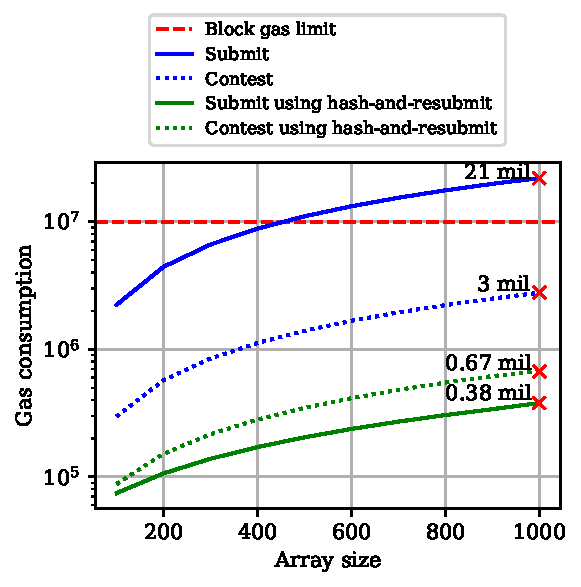
\includegraphics[width=1 \columnwidth]{figures/har-example.pdf}
\end{center}
\caption{Gas-cost reduction using the \emph{hash-and-resubmit} pattern. By
    avoiding gas-heavy storage operations, the aggregated cost of
    \textsf{submit} and \textsf{contest} is decreased significantly by 95\%.}
\label{fig:har-example}
\end{figure}

By using the \emph{hash-and-resubmit} pattern, the overall gas consumption for
\textsf{submit} and \textsf{contest} is decreased by 95\%. This
significantly affects the efficiency and applicability of the contract. Note
that, the storage implementation exceeds the Ethereum block gas
limit\footnote{As of July 2020, the Ethereum block gas limit approximates
10,000,000 gas units} for arrays of size 500 and above, contrary to the
optimized version, which consumes approximately $1/10^{th}$ of the block gas
limit for arrays of 1000 elements.

\noindent \textbf{Variations.} Now consider a variation of the above game, in
which $\pla$ calls \texttt{\proc$_1$(}$\arra$\texttt{)}, and then calls
\texttt{pickSpan(}$m, n$\texttt{)} that determines the span of $\arra$ which
can be contested. In reality, $\plb$ only needs to re-send $\arras[m:n]$ in
order to perform the comparison $\arra[m:n] < \arrb$. However, the digest of
$\arra$ is calculated by hashing the entire structure. Therefore, the
$resubmit$ phase cannot be successfully performed with $\arras[m:n]$, because
\texttt{H(}$\arra$\texttt{)} $\ne$ \texttt{H(}$\arra[m:n]$\texttt{)}.

An intuitive approach to address such scenarios in order to facilitate
selective dispatch of structure segments is to adopt different hashing schemas
that utilize constructions such as Merkle Trees (ref) or Merkle Mountain Ranges
(ref). In this variation of the pattern, which we term
\emph{merkle-hash-and-resubmit}, the signature of $\arra$ is generated by
constructing the Merkle Root of $\arra$ in contract's state. In \emph{resubmit}
phase, $\arra[m:n]$ is dispatched, accompanied by the siblings that reconstruct
the Merkle Root of $\arra$ in order to perform the variation of $\arras[m:n]$.

\begin{figure*}[h]
    \begin{center}
        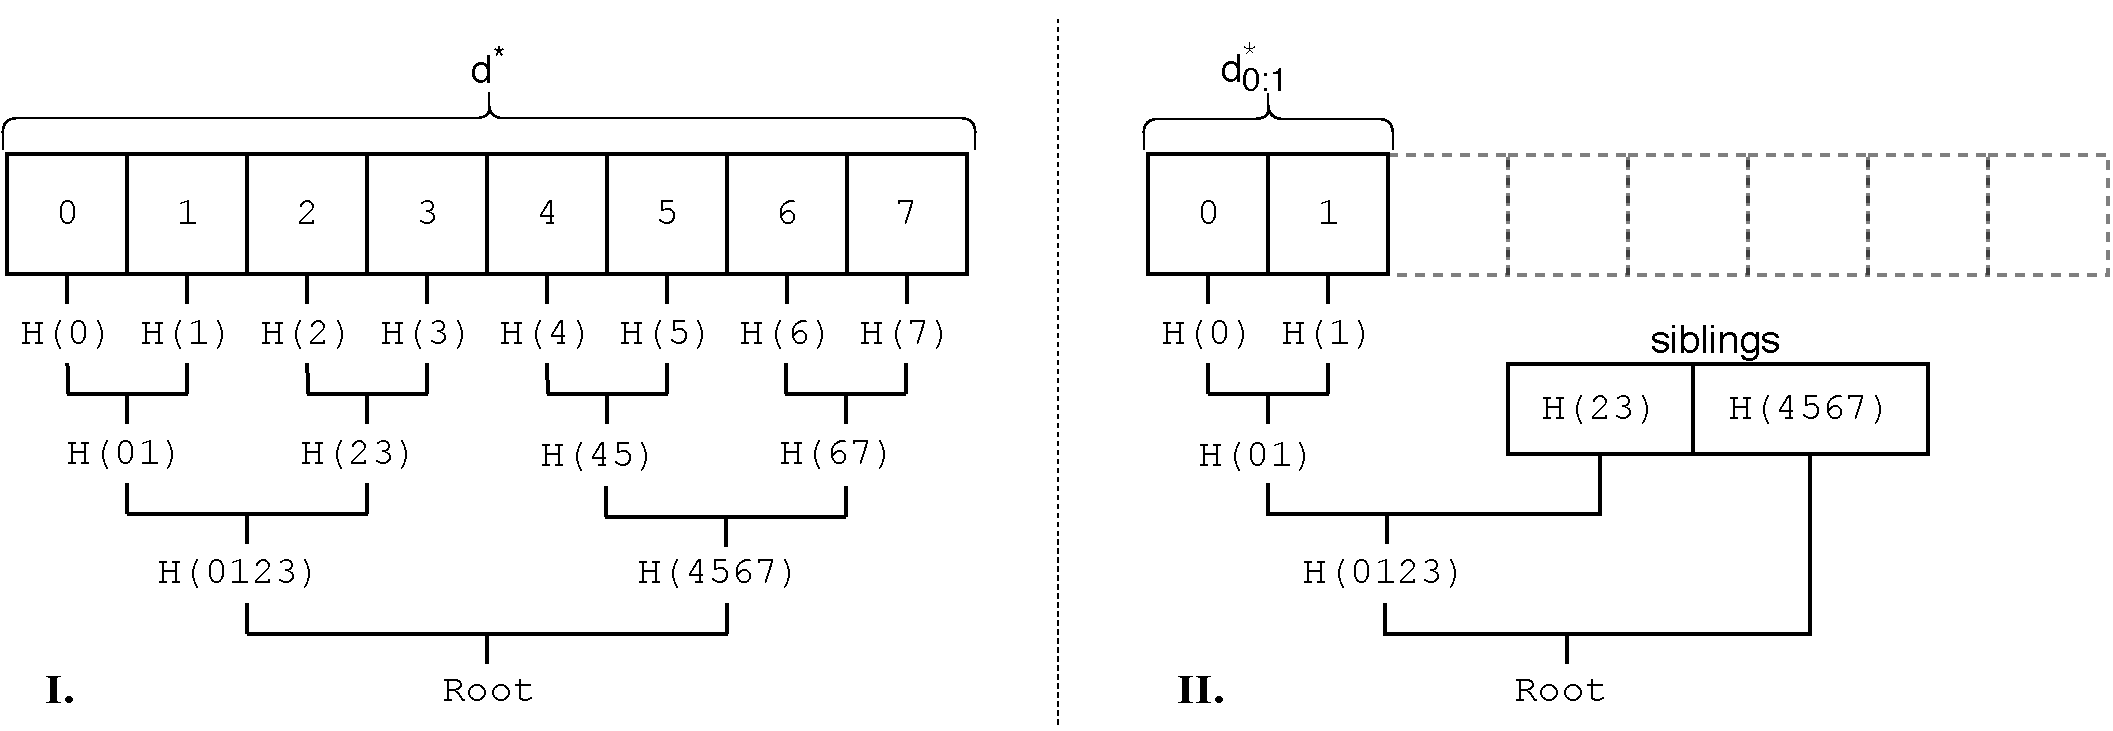
\includegraphics[width=0.8\textwidth]{figures/merkle-har.pdf}
    \end{center}
    \caption{\textbf{I.} The calculation of root in \emph{hash} phase.
    \textbf{II.} The verification of the root in \emph{resubmit} phase.
    \textsf{H}($k$) denotes the digest of element $k$. \textsf{H}($kl$) denotes the
    result of \textsf{H}(\textsf{H}($k$) $|$ \textsf{H}($l$))
}
    \label{fig:merkle-har}
\end{figure*}

This variation of the pattern removes the burden of sending redundant data,
however it implies on-chain construction and validation of the Merkle
construction. In order to construct a Merkle Tree Root for an array \textsf{a}
of size \textsf{n}, the hash function \textsf{H}($|$\textsf{a}$[n]|$) needs to
be called approximately $2^{\lceil log_2(n) + 1 \rceil}$ times for each element
of \textsf{a}. For the verification, in order to reconstruct the Merkle Tree
Root, approximately $\lceil log_2{n} \rceil$ calls to \textsf{H}(.) are needed.
The process of constructing and verifying the Merkle Tree Root is displayed in
Figure ~\ref{fig:merkle-har}.

In Solidity, hashing operations are expensive relatively to memory cost. An
invocation of \textsf{sha256}(\textsf{a}), copies the data in memory, and then
a \textsf{CALL} instruction is performed by the EVM to the pre-compiled
\textsf{sha256} contract.  In the current state of the EVM, \textsf{CALL} costs
700 gas units, and the gas paid for every additional word when expanding memory
is 3 gas units~\cite{wood}. Costs of all related operations are listed in
Table~\ref{tab:operations-gas}. Due to such a large discrepancy in gas costs,
it is more efficient to send data of size $|$\textsf{a}$|$ and perform one hash
operation \textsf{sha256}(a) than sending data of size $log_2(|\textsf{a}|)$
and perform $2^{log_2(\textsf)} \times$\textsf{sha}(1) operations. A different
cost policy applies for \textsf{keccak}~\cite{keccak}, where hashing costs 30
gas units plus 6 additional gas far each word for input data. Although the
usage of \textsf{keccak} dramatically increases the performance in comparison
with \textsf{sha256}, plain rehashing performs generally better.

\begin{table}[!h]
\begin{tabular}{|c|c|}
\hline
\textbf{Operation} & \textbf{Gas cost} \\ \hline
\textsf{load}($\data$)            & $ \data_{bytes} \times 68 $          \\ \hline
\textsf{sha256}($\data$)          & $\data_{words} \times 3 + 700 $     \\ \hline
\textsf{keccak}($\data$)          & $\data_{words} \times 6 + 30 $      \\ \hline
\end{tabular}
\caption{Gas cost of EVM operations as of June 2020.}
\label{tab:operations-gas}
\vspace*{-5mm}
\end{table}


In Table~\ref{tab:har-vs-mhar} we display the operations needed for hashing and
verifying the underlying data for both variations of the pattern as a function
of data size. In Figure~\ref{fig:har-vs-mhar} we demonstrate the gas
consumption of each variation for $\data_0$ = 10KB and $\data$ varing from $0.01
\times|\data|$ to $2\times|\data|$.

\newcommand{\mydata}{\data}

\begin{table}[h]
\begin{tabular}{|c|c|c|}
\hline
\textbf{\begin{tabular}[c]{@{}c@{}}phase per\\variance\end{tabular}} &
\textbf{\begin{tabular}[c]{@{}c@{}}plain hash\\and resubmit\end{tabular}} &
\textbf{\begin{tabular}[c]{@{}c@{}}merkle hash\\ and resubmit\end{tabular}} \\ \hline
\textbf{hash} &
\textsf{H}($\mydata$) &
\begin{tabular}[c]{@{}c@{}}
    \textsf{H}($\mydata_{elem}$) $\times\ |\mydata|$ \\ \textsf{H}(digest)
$\times\ (|\mydata|-1)$

\end{tabular} \\ \hline
\textbf{resubmit} &
\textsf{load}($\mydata$) + \textsf{H}($\mydata$) &
\begin{tabular}[c]{@{}c@{}}
    \textsf{load}($\mydata[m{:}n])$ + \\
    \textsf{load}($siblings$) + \\
    \textsf{H}($\mydata[m{:}n])$ + \\
    \textsf{H}($digest$)$\times |siblings|$
\end{tabular} \\ \hline
\end{tabular}

\caption{Summary of operations for \emph{hash-and-resubmit} pattern variations.
$\mydata$ is the product of on-chain operations and $\mydata_{elem}$ is an
element of $\mydata$. \textsf{H} is a hash function, such as \textsf{sha256}
or \textsf{keccak}, $digest$ is the product of \textsf{H}(.) and $siblings$ are
the siblings of the Merkle Tree constructed for $\mydata$.
}

\label{tab:har-vs-mhar}
\vspace*{-10mm}
\end{table}


\begin{figure}[h]
    \begin{center}
        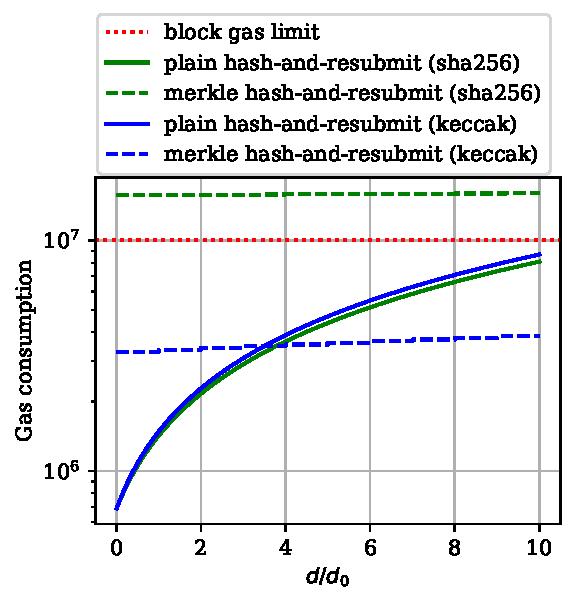
\includegraphics[width=1\columnwidth]{figures/har-vs-mhar.pdf}
    \end{center}
    \caption{Trade-offs between \emph{hash-and-resubmit} variations. In the
    vertical axis the gas consumption is displayed, and in vertical axis the
    size of $\data$ as a function of $\data_0$. The size of $d_0$ is 10KB
    bytes, and the hash function we used is pre-compiled \texttt{sha256}.}
    \label{fig:har-vs-mhar}
\end{figure}

\noindent \textbf{Consequences.} The most obvious consequence of applying the
\emph{hash-and-resubmit} pattern variations is the circumvention of storage
structures, a benefit that saves a substantial amount of gas, especially in the
cases where these structures are large. To that extend, smart contracts that
exceed the Ethereum block gas limit become practical. Furthermore, the pattern
enables off-chain transactions, significantly improving the performance of
smart contracts.

\noindent \textbf{Known uses.} To our knowledge, we are the first to combine
the notion of the transparency of the blockchain with data structures
signatures to eliminate storage variables from Solidity smart contracts by
resubmitting data.

\noindent \textbf{Enabling NIPoPoWs.} We now present how the
\emph{hash-and-resubmit} pattern can used in the context of the NIPoPoW
superlight client. Similar to the aforementioned example, the NIPoPoW verifier
adheres to a submit-and-contest-phase schema, and the inputs of the functions
are arrays that are processed on-chain.

In \emph{submit} phase, a \emph{proof} is submitted, which can be contested by
another user in \emph{contest} phase. The user that initiates the contest,
monitors the traffic of the smart contract~\cite{nipopows}. This is a logical
assumption as mentioned in the NIPoPoW paper. The input of \textsf{submit}
function includes the submit proof ($\pis$) that indicates the occurrence of an
\emph{event} ($e$) in the source chain, and the input of \textsf{contest}
function includes the contesting proof ($\pic$). A successful contest of $\pis$
is realized when $\pic$ has a better score. The process of score evaluation
which is described in ~\cite{nipopows}, is irrelevant to the pattern and
remains unchained.

In previous work~\cite{gglou}, NIPoPoW arrays are saved on-chain, resulting to
extensive storage operations that limit the applicability of the contract
considerably. In Algorithm~\ref{alg:har-nipopow} we show how hash-and-resubmit
pattern is embedded into the NIPoPoW client. In Figure~\ref{fig:har-nipopow},
we display how results of the \emph{hash-and-resubmit} implementation
differentiate from previous work for the two phases. We observe that by using
the \emph{hash-and-resubmit} pattern, we achieve to increase the performance of
the contract by reducing the gas consumption by 40\%. This is a decisive step
towards creating a practical superlight client.
\newcommand{\genesis}{\textsf{G}}

\begin{algorithm}
    \label{alg:har-nipopow}
    \caption{The \textsf{NIPoPoW} client using hash-and-resubmit pattern}
    \begin{algorithmic}[1]

    \Contract{crosschain}
    \State $\textsf{events} \gets \bot;$ $\genesis \gets \bot$
    \Function{\sf initialize}{$\genesis_{remote}$}
        \State \genesis $\gets \genesis_{remote}$
    \EndFunction
    \Function{\sf submit}{$\pis$, $e$}
        \State \textsf{require}($\pis$[0] = $\genesis$)
        \State \textsf{require}($\textsf{events$[e]$} = \bot$)
        \State \textsf{require}($\textsf{valid-interlink}(\pi)$)
        \State \textsf{DAG} $\gets$ \textsf{DAG} $\cup$ $\pis$
        \State \textsf{events$[e]$.hash} $\gets$ \textsf{H}($\pis$)
        \Comment{enable pattern}
        \State \textsf{ancestors} $\gets$ \textsf{find-ancestors()}
        \State \textsf{events$[e]$.pred} $\gets$
            \textsf{evaluate-predicate}(\textsf{ancestors}, e)
        \State \textsf{ancestors} $=$ $\bot$
    \EndFunction
    \Function{\sf contest}{$\pisa$, $\pic$, $e$}
        \Comment{provide proofs}
        \State \textsf{require}(\textsf{events$[e]$.hash} $=$ \textsf{H}($\pisa$))
        \Comment{verify $\pisa$}
        \State \textsf{require}($\pic$[0] = $\genesis$)
        \State \textsf{require}(\textsf{events}$[e]$ $\ne$ $\bot$)
        \State \textsf{require}(\textsf{valid-interlink}($\pi_{cont}$))
        \State $lca$ = \textsf{find-lca}($\pisa$, $\pic$)
        \State \textsf{require}(\textsf{score}($\pic[:lca]$)
            $>$ \textsf{score}($\pisa[:lca]$))
        \State \textsf{DAG} $\gets$ \textsf{DAG} $\cup$ $\pic$
        \State \textsf{ancestors} $\gets$ \textsf{find-ancestors}(\textsf{DAG})
        \State \textsf{events$[e]$.pred} $\gets$
            \textsf{evaluate-predicate}(\textsf{ancestors}, $e$)
        \State \textsf{ancestors} $=$ $\bot$
    \EndFunction
    \EndContract
    \vskip8pt
    \end{algorithmic}
\end{algorithm}



\begin{figure}[!h]
    \begin{center}
        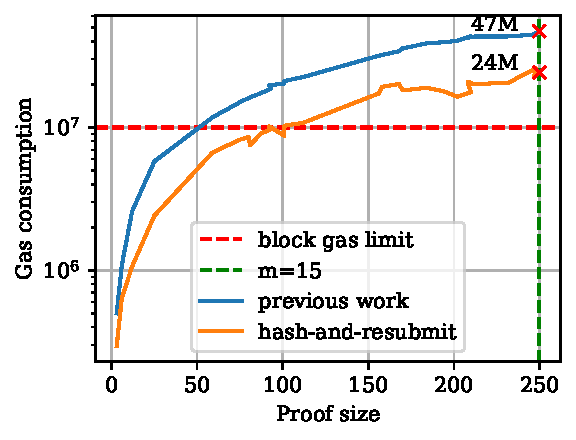
\includegraphics[width=1\columnwidth]{figures/har-nipopows.pdf}
    \end{center}
    \caption{Performance improvement using hash-and-resubmit pattern in
    NIPoPoWs related to previous work. The gas consumption decreased by
    approximately 40\%}
    \label{fig:har-nipopow}
\end{figure}
